\documentclass{article}
\usepackage{graphicx}
\usepackage{filecontents}
\usepackage{gensymb}
\usepackage{graphicx}
\usepackage[T1]{fontenc}
\usepackage[polish]{babel}
\usepackage[utf8]{inputenc}
\usepackage{gensymb}
\usepackage{siunitx}
\usepackage{amsmath}
\graphicspath{ {res/} }
 \title{Tomograf komputerowy 2D}
\date{2018\\ Marzec}
\author{Jakub Tomczak \\ Konrad Kubzdela}
\begin{document}
\maketitle

\section{Błąd średniokwadratowy}
Jako miary jakośsci użylimy średniej kwadratowej błędów, który obliczyliśmy na podstawie odchyleń wartości pikseli obrazu wyjściowego od wejściowego.

$$\sqrt{\frac{1}{n^2} \sum\limits_{i=1}^n\sum\limits_{j=1}^n (x_{ij}-y_{ij})^2}$$ 
\clearpage
\subsection{Błąd średniokwadratowy w zależności od iteracji}
\centering liczba detektorów n =50\\*
kąt rozwarcia = \ang{50}
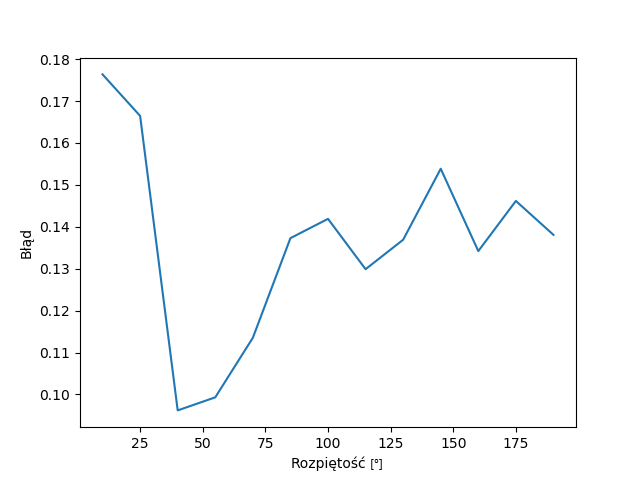
\includegraphics[width=\textwidth]{wykres3}
\centering

\subsection
 {Błąd średniokwadratowy w funkcji ilości emiterów i detektorów.}
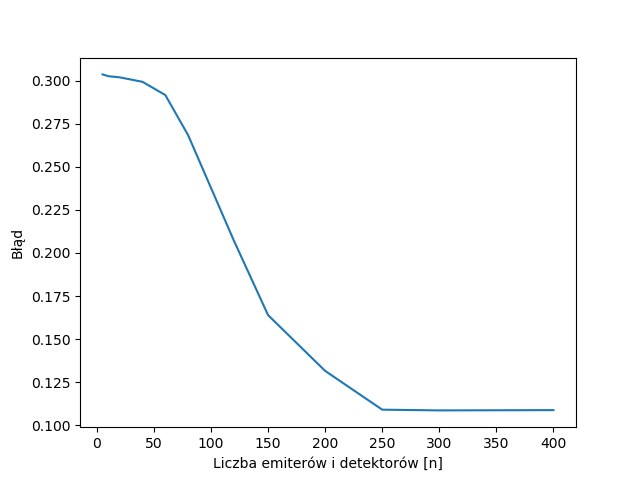
\includegraphics[width=\textwidth]{wykres}
\centering
\subsection{Błąd średniokwadratowy w zależności od zastosowanych filtrów.}
liczba detektorów n=100
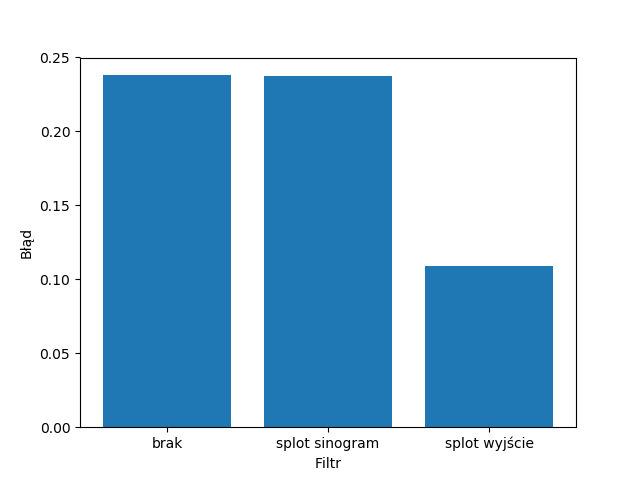
\includegraphics[width=\textwidth]{wykres2}

\subsection{Błąd średniokwadratowy w zależności od rozpiętości kątowej}
liczba detektorów n =100
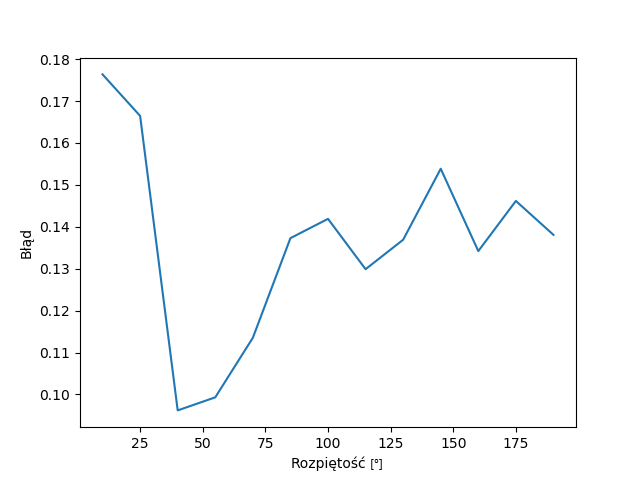
\includegraphics[width=\textwidth]{wykres3}
\centering
 
\end{document}